% kapitel4.tex
\chapter{Wagner Struktur}
\label{cha:wagnerstruktur}

In diesem Kapitel soll Theorem \ref{eq:Theorem36} genauer betrachtet werden.
Es ist, wie erwähnt, auf Wagner zurückzuführen:
\begin{theorem}\label{eq:TheoremWagner}
  Ein Graph enthält genau dann keinen \kf-Minor, wenn er ein Teilgraph eines Graphen ist, der aus planaren Graphen und Kopien von $W$ erzeugt werden kann, welche an Cliquen zusammengeführt wurden.\cite{Wag37}
\end{theorem}
Als Beispiel ist dazu in Abbildung \ref{fig:WagnerStruktur1} ein Graph $G$ zu sehen, der nicht planar ist, aber keinen \kf-Minor enthält und durch Cliquen-Summen aus dem Graph $G'$ aus Abbildung \ref{fig:WagnerStruktur2} erzeugt werden kann.
$G$ enthält demgegenüber nur planare Zusammenhangskomponente \bzw eine, die isomorph zu $W$ ist.
Einige Cliquen sind hier mit je einer Farbe hervorgehoben, sodass durch das Zusammenfügen gleichfarbiger Knoten ein Graph $G''$ erzeugt werden kann, der $G$ als Teilgraph enthält.
Zusätzlich bilden in $G''$ die roten Knoten eine Clique, in $G$ sind sie nicht adjazent.
Um einen isomorphen Graph zu erzeugen, muss $G'$ durch Cliquen-Summen erzeugt werden, da bei der Operation Kanten zwischen Cliquenknoten im Anschluss entfernt werden dürfen.
Somit kann Theorem \ref{eq:TheoremWagner} so umforumliert werden, dass jeder Graph ohne \kf-Minor durch Cliquen-Summen von planaren Graphen und Kopien von $W$ erzeugt werden kann.
Problematisch ist allerdings, dass eine Cliquen-Summe nicht festlegt, ob und welche Kanten innerhalb der Clique gelöscht werden.
Das Theorem kann aber genutzt werden, um einen Graph in seine planaren Komponenten und Kopien von $W$ aufzuteilen, sollte er keinen \kf-Minor enthalten.

\begin{figure}[H]
  \centering
  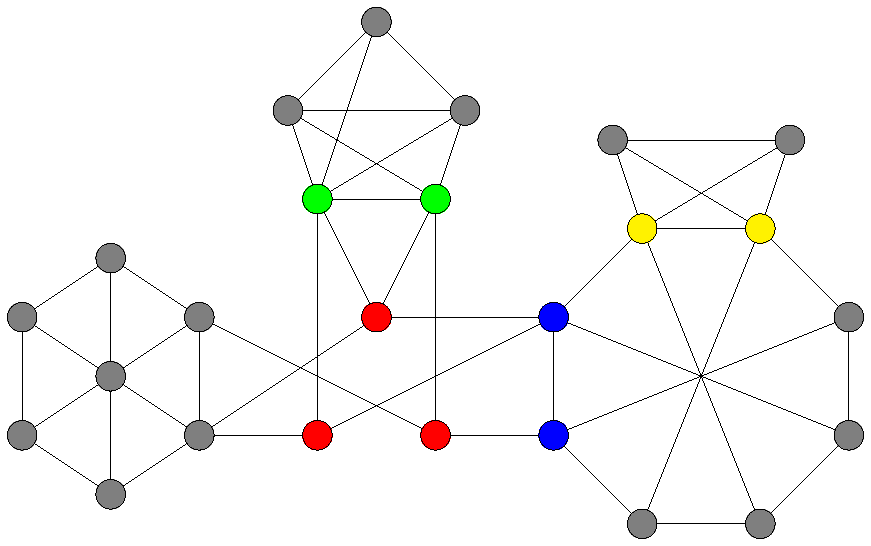
\includegraphics[width=\textwidth,height=\textheight,keepaspectratio]{bilder/WagnerTheorem1.pdf}
  \caption{Ein nicht-planarer Graph $G$, der keinen \kf-Minor enthält.}
  \label{fig:WagnerStruktur1}
\end{figure}

\begin{figure}[H]
  \centering
  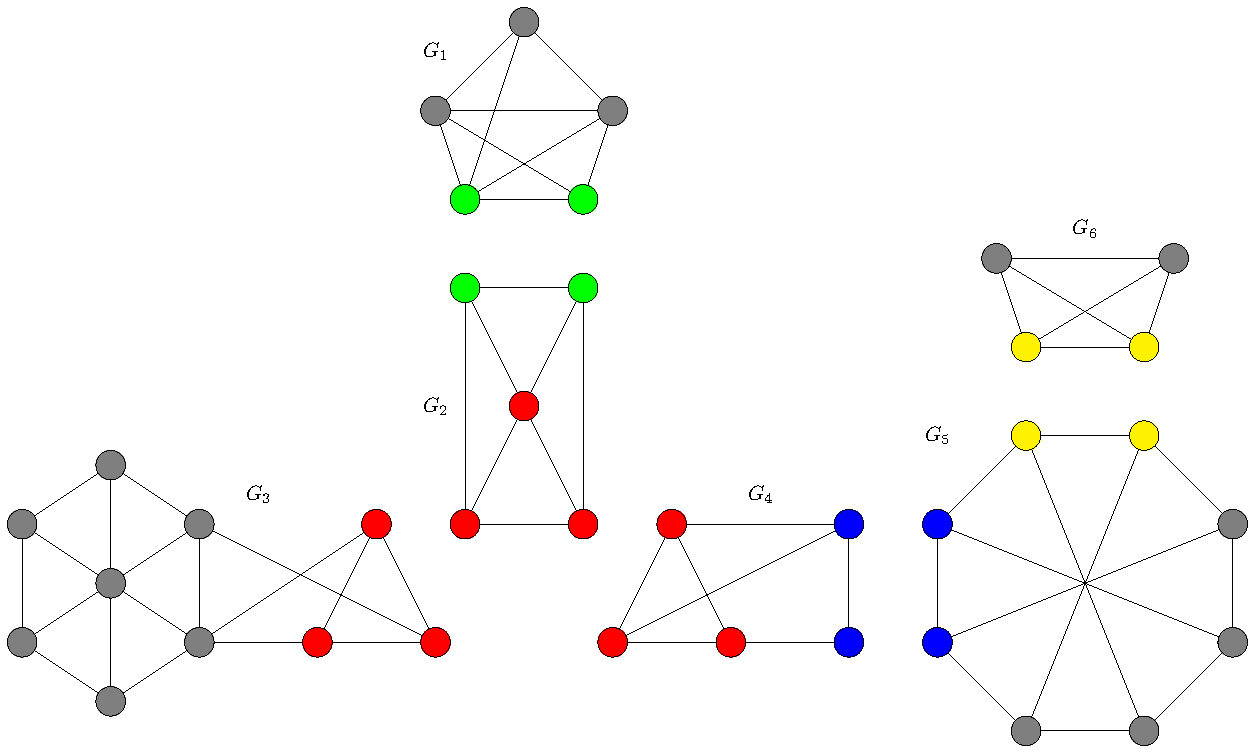
\includegraphics[width=\textwidth,height=\textheight,keepaspectratio]{bilder/WagnerTheorem2.pdf}
  \caption{Ein nicht zusammenhängender Graph $G'$, dessen Zusammenhangskomponenten planar oder isomorph zu $W$ sind.}
  \label{fig:WagnerStruktur2}
\end{figure}

In \cite{ReL08} und etwas detaillierter in \cite{ReL} stellen Reed und Li eine Möglichkeit vor, einen \kf-Minor freien Graph als Baum (oder Wald für nicht zusammenhängende Graphen) darzustellen, der die im obigen Theorem beschriebene Struktur besitzt.
Diese wird im Folgenden als \textit{Wagner-Struktur} bezeichnet und später wird gezeigt, dass der Algorithmus von Kezdy und McGuinness sie durch leichte Modifikation erzeugen kann.
Reed und Li verwandeln dazu jede Zusammenhangskomponente des Eingabegraphen in sogenannte \textit{Block-Trees}.
Die Knoten dieser Bäume seien entweder als \textit{Cliquenknoten} bezeichnet, falls sie Cliquen-Summen repräsentieren, oder als \textit{Graphknoten}, falls sie einen beliebigen Teilgraph des Eingabegraphen darstellen.


\textbf{$1$-Block-Tree}: Sei $G = (V_G, E_G)$ ein zusammenhängender, aber nicht $2$-zusammenhängender, \kf-Minor freier Graph und $T_1 = (V_T, E_T)$ der $1$-Block-Tree.
Sei $v \in V_G$ ein $(1, j)$-Separator in $G$ für $j \geq 2$ und $Z_1, ..., Z_j$ die Zusammenhangskomponenten von $G - v$.
Dann wird für jedes $Z_i$ ein Graphknoten $t_{Z_i}$ in $T_1$ angelegt, der den Teilgraph $Z_i \cup v$ enthält.
Außerdem wird ein Cliquenknoten $t_v$ angelegt, der $v$ enthält sowie Kanten zu allen $t_{Z_i}$ besitzt.
Wird das für alle $(1, j)$-Separator wiederholt, ist das Ergebnis ein Baum, dessen Graphknoten $2$-zusammenhängende Teilgraphen in $G$ repräsentieren und Cliquenknoten, die auf $(1, j)$-Separatoren in $G$ verweisen.
Ein Beispiel dazu findet sich in Abbildung \ref{fig:1-Block-Tree}.
\begin{figure}[H]
  \centering
  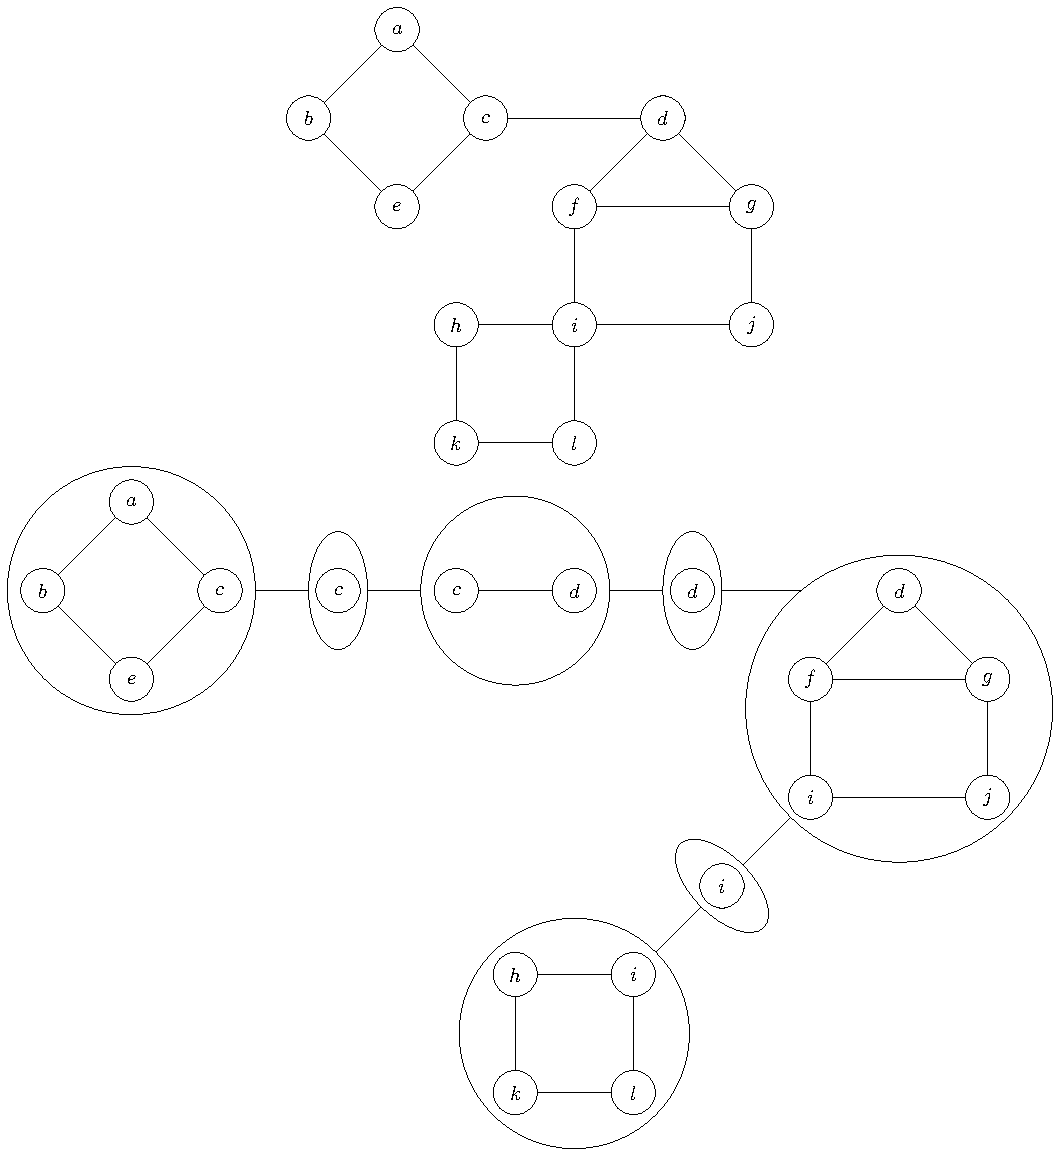
\includegraphics[width=\textwidth,height=\textheight,keepaspectratio]{bilder/1-Block-Tree.pdf}
  \caption{Oben ist ein Graph mit einem dazugehörigen $1$-Block-Tree unterhalb.
           Die Cliquenknoten sind ovalförmig und enthalten einzelne Knoten, die Graphknoten sind rund und enthalten Teilgraphen aus dem Eingabegraph.}
  \label{fig:1-Block-Tree}
\end{figure}


\textbf{$2$-Block-Tree}: Sei $G = (V_G, E_G)$ ein $2$-zusammenhängender, aber nicht $3$-zusammenhängender, \kf-Minor freier Graph und $T_2 = (V_T, E_T)$ der $2$-Block-Tree.
Bilden die Knoten $u, v \in V_G$ einen $(2, j)$-Separator in $G$ für $j \geq 2$, dann seien erneut $Z_1, ..., Z_j$ die Zusammenhangskomponenten von $G - \{u, v\}$.
Analog zum $1$-Block-Tree wird ein Cliquenknoten für den Teilgraph, der die Knoten $u$ und $v$ enthält, angelegt, der alle $Z_i \cup \{u, v\}$ als Nachbarn besitzt.
Außerdem wird die Kante $(u, v)$ sowohl in den Graph- als auch in dem Cliquenknoten hinzugefügt, falls sie nicht vorhanden ist.
Es entsteht ein Baum mit Graphknoten, der $3$-zusammenhängende Minoren von $G$ darstetllt.
Ein $2$-Block-Tree ist in Abbildung \ref{fig:2-Block-Tree} zu sehen.
Es ist zu beobachten, dass Knoten wie etwa $h$ oder $i$ Teil mehrerer Separatoren sein können und somit nicht nur in mehreren Graph-, sondern auch in mehreren Cliquenknoten enthalten sind.
\begin{figure}[H]
  \centering
  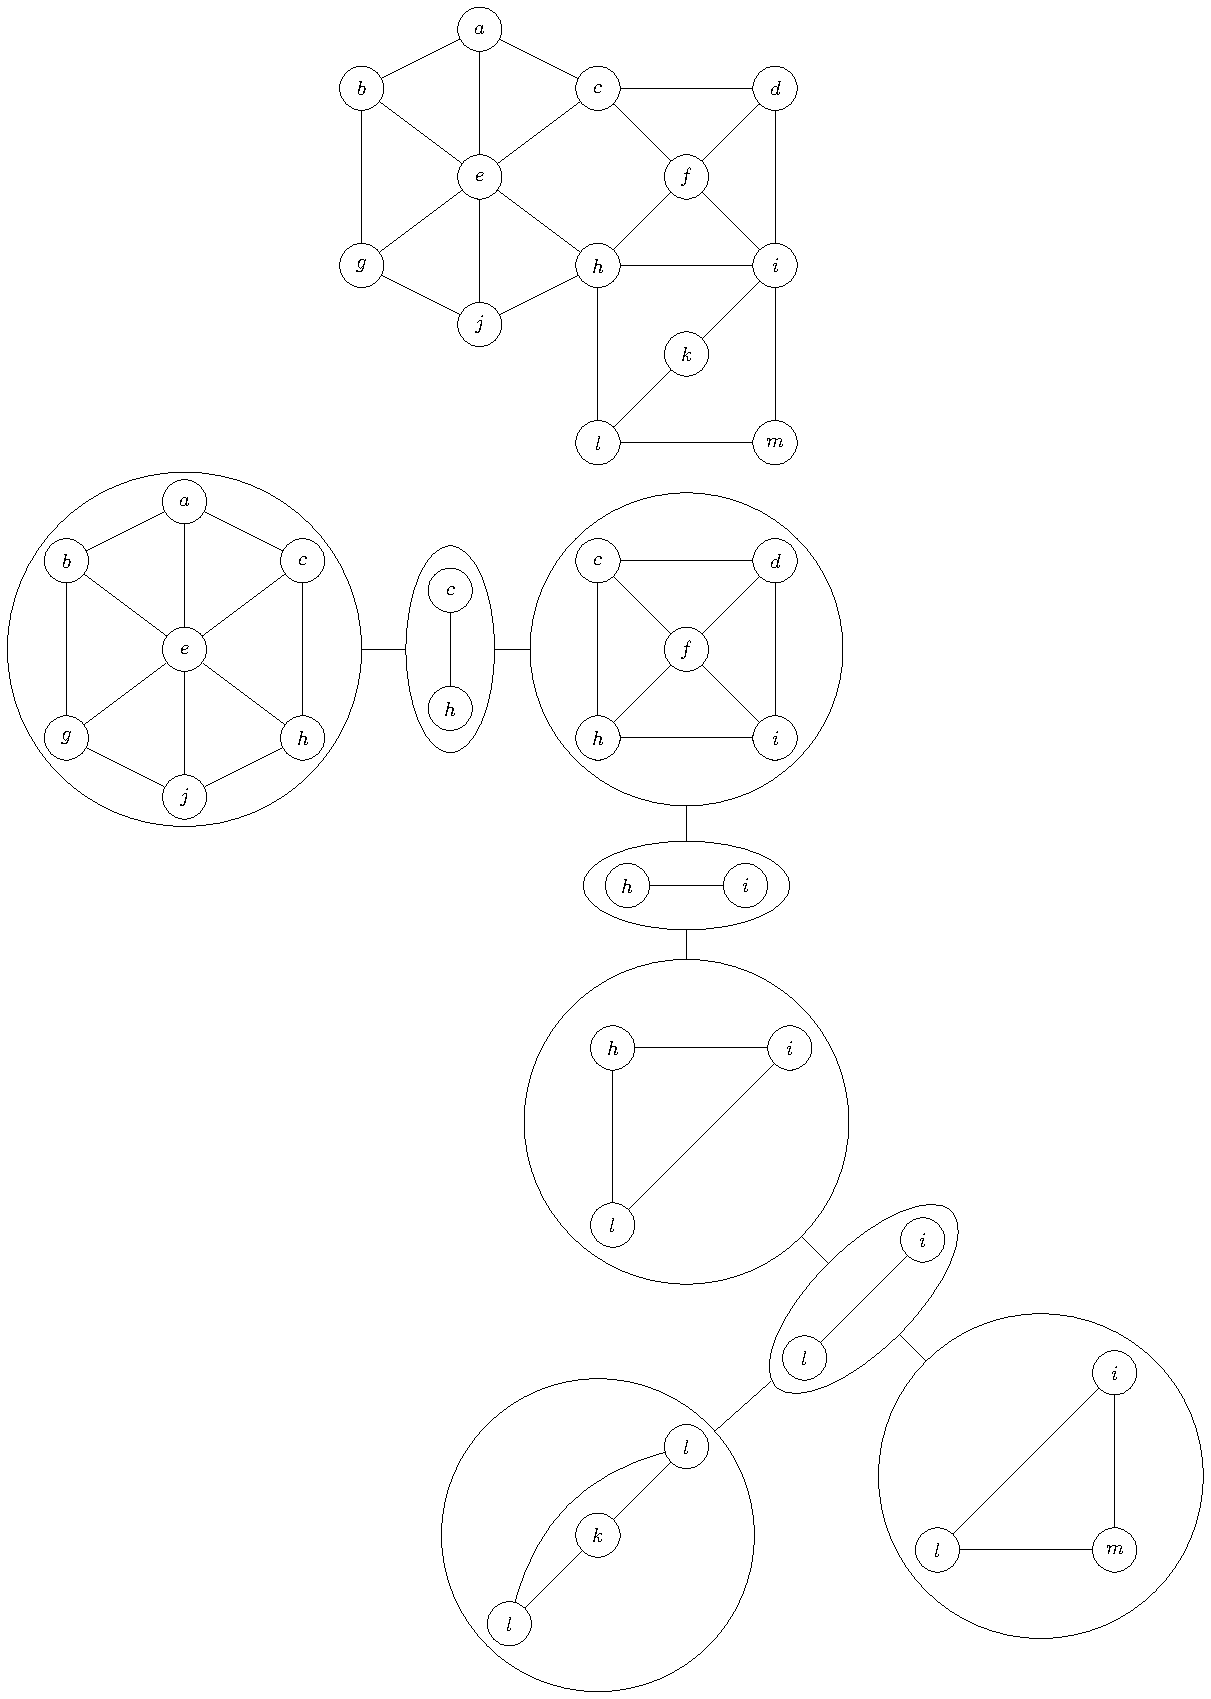
\includegraphics[width=\textwidth,height=\textheight,keepaspectratio]{bilder/2-Block-Tree.pdf}
  \caption{Oben ist ein Graph mit dazugehörigem $2$-Block-Tree unterhalb.
           Die Cliquenknoten sind ovalförmig und enthalten immer genau zwei Knoten, alle übrigen sind Graphknoten.}
  \label{fig:2-Block-Tree}
\end{figure}


\textbf{$(3, 3)$-Block-Tree}: Sei $G = (V_G, E_G)$ ein $3$-zusammenhängender, \kf-Minor freier Graph und $T_{(3, 3)} = (V_T, E_T)$ der $(3, 3)$-Block-Tree.
Enthält $G$ keinen $(3, j)$-Separator für $j \geq 3$, so besitzt $T_{(3, 3)}$ einen einzigen Graphknoten, der $G$ komplett enthält.
Sei andernfalls $C$ ein Graph, der die drei Knoten eines solchen $(3, j)$-Separatoren als Clique beinhaltet.
Dann werden Graphknoten in $T_{(3, 3)}$ für alle $Z_i \cup C$ mit $1 \leq i \leq j$ angelegt, wobei $Z_i$ die durch den Separator entstandenen Zusammenhangskomponenten sind.
Außerdem wird ein Cliquenknoten mit $C$ erzeugt, der im Baum Kanten zu allen zuvor erzeugten Graphknoten hat.
Ein Beispiel ist in Abbildung \ref{fig:33-Block-Tree} skizziert.
\begin{figure}[H]
  \centering
  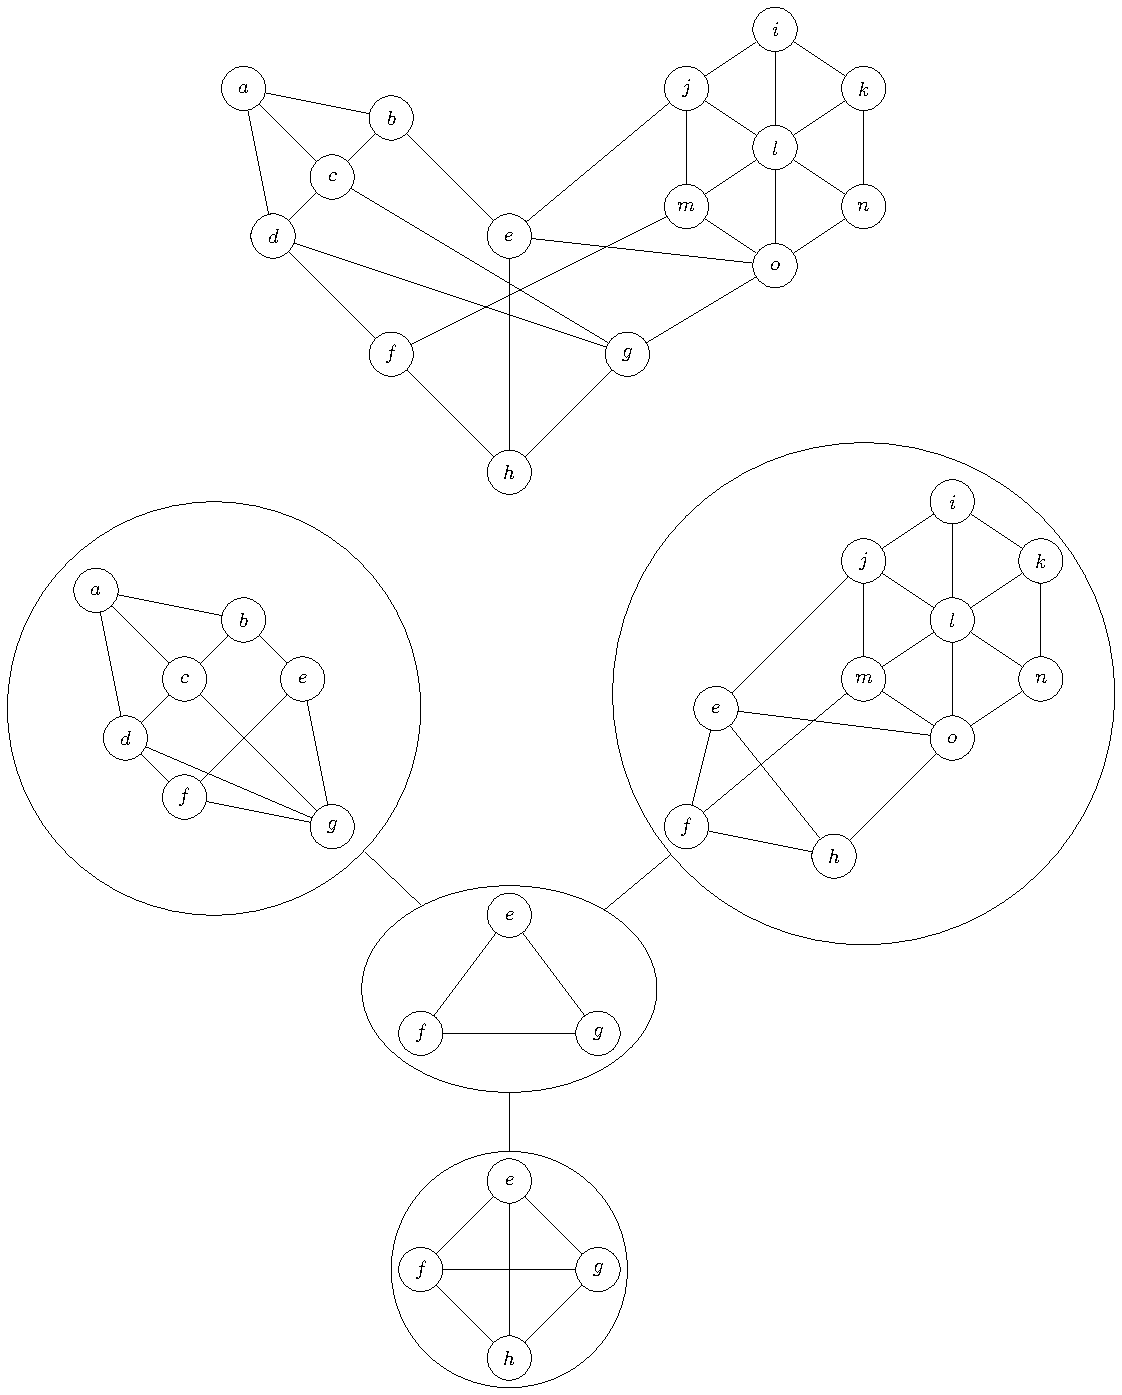
\includegraphics[width=\textwidth,height=\textheight,keepaspectratio]{bilder/33-Block-Tree.pdf}
  \caption{Ein $3$-zusammenhängender Graph mit dazugehörigem $(3, 3)$-Block-Tree.
           Der Separator wird durch ${e, f, g}$ gebildet.
           Es ist zu sehen, dass der Eingabegraph nicht planar ist, da ein \kdd-Minor enthalten ist.
           Die Graphknoten enthalten jedoch alle planare Minoren des ursprünglichen Graphs.}
  \label{fig:33-Block-Tree}
\end{figure}


Um nun aus einem schlichten nicht zusammenhängenden Graph $G$ ohne \kf-Minor eine Wagner-Struktur zu erzeugen, wird zunächst für jede Zusammenhangskomponente ein $1$-Block-Tree $T_1$ angelegt.
Jeder Graphknoten $t \in T_1$ beinhaltet einen $2$-zusammenhängenden Teilgraph $G'$ von $G$, welcher als Eingabe für einen $2$-Block-Tree $T_2$ dient.
Ist $G$ bereits $2$- \bzw $3$-zusammenhängend, kann der entsprechende Block-Tree übersprungen und $G$ direkt als Eingabe für den $2$- \bzw $(3, 3)$-Block-Tree verwendet werden.
Anschließend kann jeder $3$-zusammenhängende Teilgraph $G''$, der mit einem Graphknoten von $T_2$ assoziiert wird, als Eingabe für einen $(3, 3)$-Block-Tree verwendet werden.
Dadurch entsteht ein Baum, der zeigt, wie nach Theorem \ref{eq:TheoremWagner} der Graph $G$ aus planaren Graphen und Kopien von $W$ durch Cliquen-Summen erzeugt werden kann.
Wie zuvor angedeutet, ist zwar der Eingabegraph nicht immer eindeutig aus der Wagner-Struktur wiederherstellbar, allerdings ist die relevante Eigenschaft einer solchen Struktur vielmehr, dass sie nur für \kf-Minor freie Graphen existiert.
Scheitert der Aufbau einer Wagner-Struktur, ist der Graph nicht \kf-Minor frei.


\section{Algorithmus von Kezdy und McGuinness als Wagner-Struktur}
Im Folgenden wird die Wagner-Struktur von Reed und Li mit dem Algorithmus von Kezdy und McGuinness verglichen und dieser so modifiziert, dass er sie erzeugen kann.
Zunächst wird der Zusammenhang zwischen augmentierten Komponenten und den verschiedenen Block-Trees gezeigt.

\textbf{Behauptung:} Wird der Graph in augmentierte Komponenten aufgeteilt, sind diese genau dann isomorph zu mindestens einem Graphknoten der verschiedenen Block-Trees, wenn alle Separatoren gleich gewählt wurden.
Im Algorithmus von Kezdy und McGuinness wird der Graph in augmentierte Komponenten aufgeteilt, wenn ein $(1, 2)$-, $(2, 2)$- oder $(3, 3)$-Separator gefunden wird.
Sei $C$ ein solcher $(i, j)$-Separator, der einen zusammenhängenden Graph $G$ in genau $j$ Zusammenhangskomponenten $Z_1, ..., Z_j$ aufteilt, wenn die $i$ Knoten von $C$ aus $G$ entfernt werden.
Dann wird für ein beliebiges $k$ mit $1 \leq k \leq j$ aus dem Teilgraph $Z_k \cup C$ eine neue augmentierte Komponente erzeugt und, falls noch nicht vorhanden, aus den Knoten von $C$ in der Komponente eine Clique gebildet.
Wurde dadurch der $2$-Zusammenhang in allen Zusammenhangskomponente von $G$ hergestellt, existiert bei gleicher Wahl der Separatoren für jede augmentierte Komponente mindestens ein Graphknoten im $1$-Block-Tree, der auf einen zu dieser Komponente isomorphen Graph verweist.
Genauso gibt es für jeden Graph eines Graphknotens im $1$-Block-Tree mindestens eine augmentierte Komponente, die isomorph zu ihm ist.
Angenommen, es gäbe eine augmentierte Komponenten $G_a$, zu der es keinen Graphknoten $t$ mit assoziiertem Graph $G_t$ gibt, sodass $G_a$ und $G_t$ isomorph sind.
Dann gibt es einen $(1, 2)$-Separator $C_a$ in $G$, aus dem $G_a$ entstanden ist.
Da es kein $t$ mit einem zu $G_a$ isomorphen $G_t$ gibt, wurden keine Knoten im Block-Tree mit $C_a$ erzeugt, sodass es ebenfalls keinen Cliquenknoten mit $C_a$ gibt.
Dann wurde mindestens ein Separator $C_a'$ für den $1$-Block-Tree gewählt, wodurch die Knoten von $C_a$ so in Graphknoten enthalten sind, dass sie dort keinen Separator bilden, was der gleichen Wahl von Separatoren widerspricht.
Oder $C_a$ ist vollständig in einem Graphknoten enthalten und bildet dort einen Separator, was dem $2$-Zusammenhang des $1$-Block-Trees widerspricht.

Der Algorithmus von Kezdy und McGuinness erzeugt also zu Beginn alle Graphknoten eines $1$-Block-Trees.
Zusätzlich können die Knoten der gefundenen Separatoren gespeichert werden, um ebenfalls die Cliquenknoten zu erhalten, sodass der Algorithmus einen $1$-Block-Tree erzeugt.
Im zweiten Schritt werden die augmentierten Komponenten \bzw Graphknoten des $1$-Block-Tree in $3$-zusammenhängende augmentierte Komponenten \bzw einen $2$-Block-Tree überführt.
Analog zum vorherigen Fall gibt es für jede augmentierte Komponente, die aus einem Graphknoten des $1$-Block-Trees mit einem $(2, 2)$-Separator gebildet wird, einen isomorphen Graphknoten im $2$-Block-Tree, falls alle Separatoren gleich gewählt wurden.
Erneut können aus den Separatorknoten Cliquen gebildet und in zusätzlichen Knoten gespeichert werden, um als Ausgabe des zweiten Schrittes einen $2$-Block-Tree zu erzeugen.

Um die Graphknoten des $2$-Block-Trees in je einen $(3, 3)$-Block-Tree zu verwandeln, müssen nicht nur entsprechende Separatoren gefunden und augmentierte Komponente gebildet, sondern auch garantiert werden, dass die Graphknoten der $(3, 3)$-Block-Trees entweder planar oder isomorph zu $W$ sind und in keinem ein \kf-Minor enthalten ist.
Hier kann das Theorem \ref{eq:Theorem36} in Kombination mit dem zuvor angewendeten Planaritätstest genutzt werden, um die Struktur aufzubauen.
Sei dazu $G_t$ der Graph, der zu einem beliebigen Graphknoten $t$ im $2$-Block-Tree gehört.
$G_t$ muss $3$-zusammenhängend sein, da er als Graph vollständig in $t$ vorkommt.
Im Algorithmus von Kezdy und McGuinness wird $G_t$ nun im dritten Schritt durch einen Planaritätstest überprüft.
Wird ein \kf-Minor gefunden, ist die Wagner-Struktur ungültig und der Algorithmus terminiert.
Andernfalls kann $G_t$ planar sein - dann wird im $(3, 3)$-Block-Tree ein einzelner Graphknoten angelegt, der $G_t$ enthält und als planar markiert ist.
Letztlich kann der Planaritätstest ein \kdd-Homöomorph $S$ finden, sodass die Voraussetzungen für Theorem \ref{eq:Theorem36} gegeben sind.
Im ersten Fall von Theorem \ref{eq:Theorem36} enthält $G_t$ jedoch einen \kf-Minor, da keine Knoten von $S$ einen $(3, 3)$-Separator bilden - der Beweis dazu findet sich in Lemma \ref{eq:Lemma35}.
Damit wäre die Wagner-Struktur erneut ungültig.
Im zweiten Fall ist $G_t$ isomorph zu $W$.
Analog zum planaren Fall wird ein neuer Graphknoten im $(3, 3)$-Block-Tree angelegt, der $G_t$ enthält und entsprechend gekennzeichnet ist.
Der dritte und vierte Fall treten ein, falls drei Knoten aus $S$ einen $(3, 3)$-Separator bilden.
Kezdy und McGuinness erzeugen hier augmentierte Komponenten, die wie zuvor isomorph zu Graphknoten des $(3, 3)$-Block-Trees sein können.
Zusätzlich müssen die drei Knoten des Separators als neuer Cliquenknoten eingefügt und mit den entstandenen augmentierten Komponenten verbunden werden.
Der Algorithmus wird rekursiv auf jeden der Graphknoten angewendet, bis alle zugehörigen Teilgraphen planar oder isomorph zu $W$ sind \bzw ein \kf-Minor gefunden wurde.
Somit ist das Ergebnis des modifierten Algorithmus entweder eine Wagner-Struktur, die aus einem Wald von $1$-Block-Trees mit Graphknoten, die aus $2$-Block-Trees mit Graphknoten aus $(3, 3)$-Block-Trees bestehen und die die planaren Teilgraphen und Kopien von $W$ im Eingabegraph zeigen.
Oder es wird ein \kf-Minor als Teilgraph des Eingabegraphen gefunden, sodass die Wagner-Struktur ungültig ist, die Frage, ob ein \kf-Minor enthalten ist, jedoch in beiden Fällen eindeutig beantwortet werden kann.

% TODO Wagner-Struktur mit kf-Minoren
